\documentclass[12pt,a4paper]{article}
\linespread{1}
\usepackage[utf8]{inputenc}
\usepackage[margin=1in]{geometry}
\usepackage{amsmath}
\usepackage{amsthm}
\usepackage{amsfonts}
\usepackage{wrapfig,lipsum,booktabs}
\usepackage{ragged2e}
\usepackage{amssymb}
\usepackage[font=footnotesize,labelfont=bf]{caption}
\usepackage{subcaption}
\usepackage[usenames, dvipsnames]{color}
\usepackage{graphicx}
\usepackage{float}
\usepackage{hhline}
\usepackage{tabularx}
\usepackage[citestyle=authoryear, bibstyle=authoryear,backend=biber]{biblatex}
\DeclareUnicodeCharacter{8208}{-}

\newtheorem{theorem}{Theorem}

\newcommand{\rojo}{\textcolor{red}}
\newcommand{\azul}{\textcolor{blue}}

\bibliography{ref.bib}
\title{Outlining a Posterior-Approximating HMCMC Algorithm}

\begin{document}
\maketitle
\section{Brief Intro}
We would like to design an MCMC algorithm that combines Hamiltonian MCMC (HMCMC) \parencite{neal_mcmc_2012,betancourt_geometric_2014,betancourt_conceptual_2017} and the approximate posterior + refinement approach of the Shrinking Bullseye \parencite{conrad_accelerating_2015}.

The basic skeleton of an HMCMC algorithm procedes as follows:
\begin{enumerate}
\item Consider the sampler at point $\vec{q}_n$ in parameter space with posterior density $\pi(\vec{q} | \vec{y})$ where $\vec{y}$ is the observed data (supressed going forward) .
\item Draw a momentum vector $\vec{p}_n$ from the distribution $\pi(\vec{p} | \vec{q} ) = \text{N}(\vec{p} |0, M)$ where $M$ is the mass matrix (in vanilla HMCMC this is usually chosen to be the covariance matrix of $\pi(\vec{q}|\vec{y})$ but for Riemanian HMCMC I believe one uses the Hessian of $\pi(\vec{q})$ with respect to $\vec{q}$ evaluated at $\vec{q}_n$, or something similar).
\item We then numerically integrate the following Hamiltonian with step size $h$ for $s$ steps (the integration time $sh$ is a free parameter for the sampler, and needs to be chosen wisely based on the geometry of the posterior), with initial conditions $(\vec{q}_n, \vec{p}_n)$:
\begin{equation}
\begin{split}
\dot{\vec{q}} &= M^{-1} \vec{p} \\
\dot{\vec{p}} &= - \nabla ln(\pi(\vec{q}))\\
\end{split}
\end{equation}
\item This integration is typically done by the leapfrog method (see Appendix), but any other \textit{symplectic} numerical integrator will work.
\item After integrating to time $sh$ the candidate points $q_{n+1}, p_{n+1}$ (supressing vector notation) are set as $q_{n+sh}, p_{n+sh}$.  To make the process reversible we need to now negate $p_{n+1}$, so our candidate points are $q_{n+1}, -p_{n+1}$.  Then the candidate $q_{n+1}$ gets plugged into the usual Metropolis accept/reject probability.  Doing a Metropolis accept/reject would not be necessary if we could integrate (1) without error, but due to the error in (2) we would get biased estimates without the Metropolis step.
\end{enumerate}

\section{Testing Approximation Methods}
Based on my criteria (see Appendix) and conversation with Ian Grooms (see update from 6/2) I identified two approximating algorithms to compare: (1) Local Quadratic Regression (LQR) and (2) radial basis functions (specifically Thin Plate Splines, TPS).  This are both gridless methods, so are well-suited to ad hoc additions to the approximating set $S$.  Here I implement both and compare their performance (the TPS was implemented with no low-rank approximation, as it reduced approximation quality substantially without providing a substantial computational speedup).

For comparison of performance I used the test density function:
\begin{equation}
\pi(x,y) = \text{Exp} \left( -P*(A*x^2*y^2 + x^2 + y^2 - B*x*y - C*x - C*y) \right)
\end{equation}
With $A = C = 1$, $ B =10$ and $ P = 0.05$ (Fig. 1).  For gradient calculations I used the NumPy \texttt{gradient()} function, which computes the gradient by central differences.  It should be noted that for both LQR and TPS the gradient can be computed by hand, but it was simpler in implementation to just use central differences for now.  To compare the methods I fit them with 300 points chosen uniformly over the square $[-15,15] \times [-15,15]$ and computed the gradient at 1e5 gridpoints over the square $[-6,6] \times [-6,6]$.  Letting $\hat{\pi}_i$ denote the approximation from method $i$, I computed the max gradient error as:
\[
\epsilon_i = \frac{ \text{max}_{j} \left( \Vert \nabla \hat{\pi}_i(\vec{x}^{(j)}) - \nabla \pi(\vec{x}^{(j)})  \Vert \right) } { \text{max}_j \left( \Vert \nabla \pi(\vec{x}^{(j)}) \Vert \right) }
\]
Where the max's are taken over the grid points $\vec{x}^{(j)}$. I similarly computing a max function error:
\[
e_i = \frac{ \text{max}_{j} \left( \Vert \hat{\pi}_i(\vec{x}^{(j)}) - \pi(\vec{x}^{(j)})  \Vert \right) } { \text{max}_j \left( \Vert \pi(\vec{x}^{(j)}) \Vert \right) }
\]

The thin plate splines fared substantially better, with $e_{\text{TPS}} = 0.319$ and $\epsilon_{\text{TPS}} = 0.826$ compared to $e_{\text{LQR}} = 0.596$ and $\epsilon_{LQR} = 57.9$.  This was calculated with a TPS smoothness parameter $\lambda = 1e-7$.  To asses how varying this parameter changed the TPS fit I re-computed $e_{\text{TPS}}$ and $\epsilon_{\text{TPS}}$ for each $\lambda \in [1e-10, 1e-7,1e-4, 1e-1, 1, 10, 100]$.  Virtually no effect of varying $\lambda$ was detected on either measure of error, however, for all values of $\lambda$ $e_\text{TPS} = 1.105$ and $\epsilon_\text{TPS} = 0.826$ with any differences being on the order of machine precision.

\begin{figure}
\centering
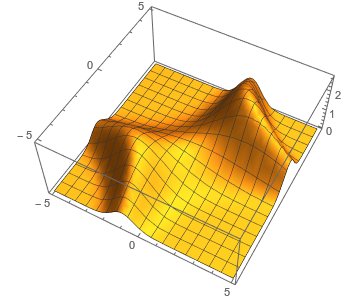
\includegraphics[scale=.6]{./Figs/test_dense.png}
\caption{The test density function in (3) with $A = 1, B =10, C = 1, P = 0.05$}
\end{figure}

I also tested how the gradient error might effect Hamiltonian dynamics when numerically integrated with leapfrog.  I chose a random initial, 2D position and momentum vector uniformly from the square $[-6,6] \times [-6,6]$, and then integrated forward for a random number of steps from 10 to 100, with fixed step size $h = 1e-5$.  I repeated this for 100 such initial conditions with the test density, as well as the LQR and TPS approximated densities.  I calculated the path error for method $i$ as $\rho_i = \frac{ \sum\limits_s \Vert q_i^{(s)} - q^{(s)} \Vert }{ \sum\limits_s \Vert q^{(s)} - q^{(s-1)} \Vert }$, $q_i^{(s)}$ is the $s^{\text{th}}$ leapfrog step for $V(x)$ approximated by method $i$, and $q^{(s)}$ is same for the ``true'' $V(x)$.  This is effectively the path integral of the leapfrog error normalized by the arc length of the true s-step forward integration.  Normalizing by arc length doesn't give a sense of how the error might behave in the long-time, but intuitively one expects the error to behave fairly poorly in the long time anyways so I wasn't as interested in measuring it.  My hope here is to instead get a sense of how badly the approximated potentials effect the Hamiltonian dynamics ``on average''; if both methods behave similarly on average I may then dig into the long-time error to see if there's an important difference there.

Averaging over the random initial conditions and step sizes we get $E[\rho_\text{LQR}] = 1.09$ and $\text{Var}[\rho_\text{LQR}] = 0.193$, while for TPS we get $E[\rho_\text{TPS}] = 0.372$ and $\text{Var}[\rho_\text{TPS}] = 0.398$.  The high variance of the TPS path error was surprising to me, although looking at the histograms of the observed error (Fig. 2) we see that the TPS approximated potential does generally perform better than the LQR approximation.  It does, however, appear that both methods had a small number of equally bad initial conditions or step sizes resulting in atypically large error.  I'm guessing that these were a particularly sensistive IC or chaotic region for the Hamiltonians.

\begin{figure}
\centering
\begin{tabular}{cc}
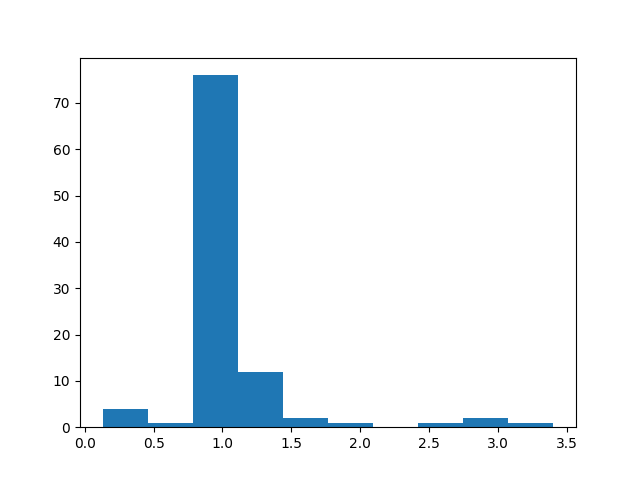
\includegraphics[scale=.5]{./Figs/lqr_ham_hist.png} & 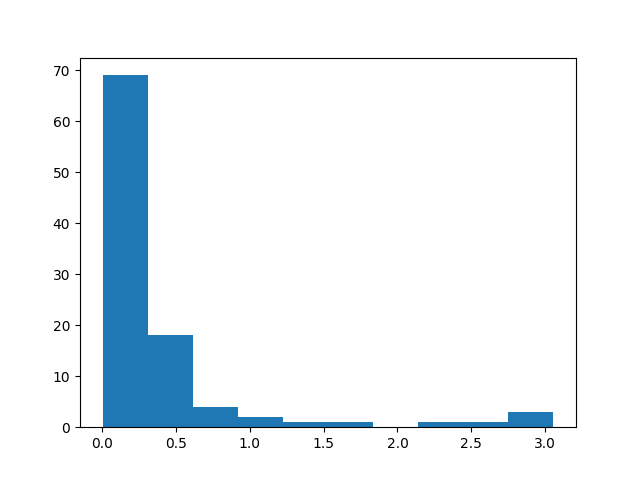
\includegraphics[scale=.5]{./Figs/tps_ham_hist.png}\\
(a) & (b)\\
\end{tabular}
\caption{Histogram of path errors for (a) the LQR approximated potential and (b) the TPS approximated potential}
\end{figure}

\section{First Steps towards an Approximate HMCMC}
Based on these results I decided to go ahead with drafting a Hamiltonian MCMC sampler using the TPS approximated posterior.  Currently the steps of this algorithm are very similar to the Shrinking Bullseye:
\begin{enumerate}
\item Starting at point $x$ we propose a point $x'$ by numerically integrating a Hamiltonian system on a potential energy surface $V(q) = -\text{ln}(\hat{\pi}(q)$ with a random initial momentumand quadratic kinetic energy (ie. $K(p) = p^T M P$ where $M$ is a mass matrix).
\item To check if $S$ requires additional points we pool the $N$ nearest points to every step in the path from Step 1.  That is, let $q^{i}$ be the $i^{\text{th}}$ step where $i = 1,...,s$ in the Leapfrog integration from Step 1, then $B_N(q^{(i)})$ are its $N$ nearest neighbors.  We then take $B = \bigcup\limits_{i=1}^{s}B_N(q^{i})$.
\item Now perform some kind of cross validation by repeating Step 1 with $\hat{\pi}$ now approximated using $S/B \cup B_l$ where $B_l$ is a random subset $B_l \subset B$ to get $K$ CV candidate points $x_k'$.  Evaluate the acceptance probability $\alpha(x,x_k')$ for each CV candidate, if $\text{max}_k \alpha(x, x_k') - \text{min}_k \alpha(x, x_k') > \epsilon$ where $\epsilon$ is some preset tolerance then we add points to $S$.  IF $\text{max}_k \alpha(x, x_k') - \text{min}_k \alpha(x, x_k') < \epsilon$ then we add no refinements.
\item  If refinements have been performed go to Step 1 and repeat from there, otherwise proceed to accept $x'$ with probability $\alpha(x,x')$
\end{enumerate}
The issue I'm hitting right now is the refinements, it's pretty expensive to just fit a fresh TPS for each CV fold of B so the algorithm would be extremely slow.  I've found some stuff on rank one updates of the coefficients that will bring the cost of fitting a TPS down from $\mathcal{O}(n^3)$ to $\mathcal{O}(n^2)$, since I'm working with around $n = 300$ interpolating points this should be a pretty big speedup.

\section{Goals for Next Week}
\begin{itemize}
\item Implementing rank one updates for the refinement step of the HMCMC with Approximated Posterior
\item Polish up the variance reduction paper, still needs a discussion section so that's my immediate goal.
\end{itemize}

\section{Appendix: Approximation Criteria}
The key feature in the Shrinking Bullseye is the inclusion of the refinements to the set of samples $S$ and $\pi(S)$ used for approximating the posterior density $\pi()$.  Thinking about adapting their basic scheme (including the refinements) to HMCMC I identified the following criteria that an approximation method for $\pi()$ should satisfy to be a good candidate for the algorithm:
\begin{enumerate}
\item The approximation must be good for both $\pi$ and $\nabla \pi$, and our interpolant must be at least once differentiable anywhere in the support of $\pi$ (twice if we’d like to do Riemanian HMCMC). Furthermore it must be straightforward or cheap to evaluate $\nabla \pi$ since we have to do so twice during a single evaulation of (2), and we are performing $s$ such evaluations per step of the sampler so total that’s $2s$ gradient evaluations per candidate proposal.
\item The approximation has to be amenable to refinements. Whatever interpolation scheme  we use, it must allow us to test for refinements (ideally through something like the cross-validation approach in the Shrinking Bullseye) as well as add new points to the interpolating data set on an ad hoc basis (ie. whenever and wherever the refinement criteria is triggered).
\item  The Hamiltonian dynamics induced by the approximation  need to be similar enough to $\pi$ that the candidates proposed are actually good. Following Betancourt’s “Conceptual Introduction to Hamiltonian Monte Carlo”, our interpolant needs to approximate the true posterior well on its typical set.
\end{enumerate}

\section{Appendix: Leapfrog Method}
One step in the integration of (1) using the leapfrog with step-size $h$ takes the form:
\begin{equation}
\begin{split}
\vec{p}_{t+h/2} &= \vec{p}_t - (\frac{h}{2})  \nabla ln(\pi(\vec{q_t}))\\
\vec{q}_h &= \vec{q}_t + (h)M^{-1} \vec{p}_{t+h/2} \\
\vec{p}_h &= \vec{p}_{t+h/2} - (\frac{h}{2})  \nabla ln(\pi(\vec{q_{t+h}})) \\
\end{split}
\end{equation}

\printbibliography

\end{document}


%%% Local Variables:
%%% mode: latex
%%% TeX-master: t
%%% End:
